% Options for packages loaded elsewhere
\PassOptionsToPackage{unicode}{hyperref}
\PassOptionsToPackage{hyphens}{url}
\documentclass[
]{book}
\usepackage{xcolor}
\usepackage{amsmath,amssymb}
\setcounter{secnumdepth}{5}
\usepackage{iftex}
\ifPDFTeX
  \usepackage[T1]{fontenc}
  \usepackage[utf8]{inputenc}
  \usepackage{textcomp} % provide euro and other symbols
\else % if luatex or xetex
  \usepackage{unicode-math} % this also loads fontspec
  \defaultfontfeatures{Scale=MatchLowercase}
  \defaultfontfeatures[\rmfamily]{Ligatures=TeX,Scale=1}
\fi
\usepackage{lmodern}
\ifPDFTeX\else
  % xetex/luatex font selection
\fi
% Use upquote if available, for straight quotes in verbatim environments
\IfFileExists{upquote.sty}{\usepackage{upquote}}{}
\IfFileExists{microtype.sty}{% use microtype if available
  \usepackage[]{microtype}
  \UseMicrotypeSet[protrusion]{basicmath} % disable protrusion for tt fonts
}{}
\makeatletter
\@ifundefined{KOMAClassName}{% if non-KOMA class
  \IfFileExists{parskip.sty}{%
    \usepackage{parskip}
  }{% else
    \setlength{\parindent}{0pt}
    \setlength{\parskip}{6pt plus 2pt minus 1pt}}
}{% if KOMA class
  \KOMAoptions{parskip=half}}
\makeatother
\usepackage{color}
\usepackage{fancyvrb}
\newcommand{\VerbBar}{|}
\newcommand{\VERB}{\Verb[commandchars=\\\{\}]}
\DefineVerbatimEnvironment{Highlighting}{Verbatim}{commandchars=\\\{\}}
% Add ',fontsize=\small' for more characters per line
\usepackage{framed}
\definecolor{shadecolor}{RGB}{248,248,248}
\newenvironment{Shaded}{\begin{snugshade}}{\end{snugshade}}
\newcommand{\AlertTok}[1]{\textcolor[rgb]{0.94,0.16,0.16}{#1}}
\newcommand{\AnnotationTok}[1]{\textcolor[rgb]{0.56,0.35,0.01}{\textbf{\textit{#1}}}}
\newcommand{\AttributeTok}[1]{\textcolor[rgb]{0.13,0.29,0.53}{#1}}
\newcommand{\BaseNTok}[1]{\textcolor[rgb]{0.00,0.00,0.81}{#1}}
\newcommand{\BuiltInTok}[1]{#1}
\newcommand{\CharTok}[1]{\textcolor[rgb]{0.31,0.60,0.02}{#1}}
\newcommand{\CommentTok}[1]{\textcolor[rgb]{0.56,0.35,0.01}{\textit{#1}}}
\newcommand{\CommentVarTok}[1]{\textcolor[rgb]{0.56,0.35,0.01}{\textbf{\textit{#1}}}}
\newcommand{\ConstantTok}[1]{\textcolor[rgb]{0.56,0.35,0.01}{#1}}
\newcommand{\ControlFlowTok}[1]{\textcolor[rgb]{0.13,0.29,0.53}{\textbf{#1}}}
\newcommand{\DataTypeTok}[1]{\textcolor[rgb]{0.13,0.29,0.53}{#1}}
\newcommand{\DecValTok}[1]{\textcolor[rgb]{0.00,0.00,0.81}{#1}}
\newcommand{\DocumentationTok}[1]{\textcolor[rgb]{0.56,0.35,0.01}{\textbf{\textit{#1}}}}
\newcommand{\ErrorTok}[1]{\textcolor[rgb]{0.64,0.00,0.00}{\textbf{#1}}}
\newcommand{\ExtensionTok}[1]{#1}
\newcommand{\FloatTok}[1]{\textcolor[rgb]{0.00,0.00,0.81}{#1}}
\newcommand{\FunctionTok}[1]{\textcolor[rgb]{0.13,0.29,0.53}{\textbf{#1}}}
\newcommand{\ImportTok}[1]{#1}
\newcommand{\InformationTok}[1]{\textcolor[rgb]{0.56,0.35,0.01}{\textbf{\textit{#1}}}}
\newcommand{\KeywordTok}[1]{\textcolor[rgb]{0.13,0.29,0.53}{\textbf{#1}}}
\newcommand{\NormalTok}[1]{#1}
\newcommand{\OperatorTok}[1]{\textcolor[rgb]{0.81,0.36,0.00}{\textbf{#1}}}
\newcommand{\OtherTok}[1]{\textcolor[rgb]{0.56,0.35,0.01}{#1}}
\newcommand{\PreprocessorTok}[1]{\textcolor[rgb]{0.56,0.35,0.01}{\textit{#1}}}
\newcommand{\RegionMarkerTok}[1]{#1}
\newcommand{\SpecialCharTok}[1]{\textcolor[rgb]{0.81,0.36,0.00}{\textbf{#1}}}
\newcommand{\SpecialStringTok}[1]{\textcolor[rgb]{0.31,0.60,0.02}{#1}}
\newcommand{\StringTok}[1]{\textcolor[rgb]{0.31,0.60,0.02}{#1}}
\newcommand{\VariableTok}[1]{\textcolor[rgb]{0.00,0.00,0.00}{#1}}
\newcommand{\VerbatimStringTok}[1]{\textcolor[rgb]{0.31,0.60,0.02}{#1}}
\newcommand{\WarningTok}[1]{\textcolor[rgb]{0.56,0.35,0.01}{\textbf{\textit{#1}}}}
\usepackage{longtable,booktabs,array}
\usepackage{calc} % for calculating minipage widths
% Correct order of tables after \paragraph or \subparagraph
\usepackage{etoolbox}
\makeatletter
\patchcmd\longtable{\par}{\if@noskipsec\mbox{}\fi\par}{}{}
\makeatother
% Allow footnotes in longtable head/foot
\IfFileExists{footnotehyper.sty}{\usepackage{footnotehyper}}{\usepackage{footnote}}
\makesavenoteenv{longtable}
\usepackage{graphicx}
\makeatletter
\newsavebox\pandoc@box
\newcommand*\pandocbounded[1]{% scales image to fit in text height/width
  \sbox\pandoc@box{#1}%
  \Gscale@div\@tempa{\textheight}{\dimexpr\ht\pandoc@box+\dp\pandoc@box\relax}%
  \Gscale@div\@tempb{\linewidth}{\wd\pandoc@box}%
  \ifdim\@tempb\p@<\@tempa\p@\let\@tempa\@tempb\fi% select the smaller of both
  \ifdim\@tempa\p@<\p@\scalebox{\@tempa}{\usebox\pandoc@box}%
  \else\usebox{\pandoc@box}%
  \fi%
}
% Set default figure placement to htbp
\def\fps@figure{htbp}
\makeatother
\setlength{\emergencystretch}{3em} % prevent overfull lines
\providecommand{\tightlist}{%
  \setlength{\itemsep}{0pt}\setlength{\parskip}{0pt}}
\usepackage[]{natbib}
\bibliographystyle{plainnat}
\usepackage{booktabs}
\usepackage{bookmark}
\IfFileExists{xurl.sty}{\usepackage{xurl}}{} % add URL line breaks if available
\urlstyle{same}
\hypersetup{
  pdftitle={Times Series Part 1},
  pdfauthor={Samuel Rowe adapted from Wooldridge (2011)},
  hidelinks,
  pdfcreator={LaTeX via pandoc}}

\title{Times Series Part 1}
\author{Samuel Rowe adapted from Wooldridge (2011)}
\date{2025-09-19}

\begin{document}
\maketitle

{
\setcounter{tocdepth}{1}
\tableofcontents
}
\begin{Shaded}
\begin{Highlighting}[]
\NormalTok{bookdown}\SpecialCharTok{::}\FunctionTok{render\_book}\NormalTok{()}
\end{Highlighting}
\end{Shaded}

\chapter*{Overview}\label{overview}
\addcontentsline{toc}{chapter}{Overview}

Topics:

\begin{enumerate}
\def\labelenumi{\arabic{enumi}.}
\tightlist
\item
  Static Model
\item
  Finite Distributed Lag Model
\item
  Time Trends
\item
  Seasonality
\item
  AR(1) Model
\end{enumerate}

\chapter{Static Models}\label{static-models}

\section{Static Philips Curve}\label{static-philips-curve}

\textbf{Lesson:} Problematic analysis with a static model between inflation and
unemployment

Set the Time Series

\begin{Shaded}
\begin{Highlighting}[]
\NormalTok{cd }\StringTok{"/Users/Sam/Desktop/Econ 645/Data/Wooldridge"}
\KeywordTok{use}\NormalTok{ phillips.dta, }\KeywordTok{clear}
\KeywordTok{tsset} \FunctionTok{year}\NormalTok{, }\FunctionTok{yearly}
\KeywordTok{reg}\NormalTok{ inf unem }\KeywordTok{if} \FunctionTok{year}\NormalTok{ \textless{} 1997}
\end{Highlighting}
\end{Shaded}

\begin{verbatim}
/Users/Sam/Desktop/Econ 645/Data/Wooldridge

        time variable:  year, 1948 to 2003
                delta:  1 year

      Source |       SS           df       MS      Number of obs   =        49
-------------+----------------------------------   F(1, 47)        =      2.62
       Model |  25.6369575         1  25.6369575   Prob > F        =    0.1125
    Residual |   460.61979        47  9.80042107   R-squared       =    0.0527
-------------+----------------------------------   Adj R-squared   =    0.0326
       Total |  486.256748        48  10.1303489   Root MSE        =    3.1306

------------------------------------------------------------------------------
         inf |      Coef.   Std. Err.      t    P>|t|     [95% Conf. Interval]
-------------+----------------------------------------------------------------
        unem |   .4676257   .2891262     1.62   0.112    -.1140213    1.049273
       _cons |    1.42361   1.719015     0.83   0.412    -2.034602    4.881822
------------------------------------------------------------------------------
\end{verbatim}

Our result do not suggest a trade off between inflation and unemployment, and
potentially suggest a positive relationship. This is likely a misspecified
model and does not best describe the short-run trade-off between inflation
and unemployment. We'll look at an augmented Phillips curve that better
describes the relationship.

Let's graph our time series

\begin{Shaded}
\begin{Highlighting}[]
\KeywordTok{twoway} \KeywordTok{line}\NormalTok{ inf }\FunctionTok{year}\NormalTok{, }\BaseNTok{title}\NormalTok{(}\StringTok{"Annual Inflation Rate"}\NormalTok{)}
\KeywordTok{graph} \KeywordTok{export} \StringTok{"/Users/Sam/Desktop/Econ 645/Stata/week\_10\_inf\_line.png"}\NormalTok{, }\KeywordTok{replace}
\NormalTok{![Line }\KeywordTok{graph} \KeywordTok{of}\NormalTok{ inflation](week\_10\_inf\_line.png)}
\end{Highlighting}
\end{Shaded}

We can use tsline as well.

\begin{Shaded}
\begin{Highlighting}[]
\KeywordTok{tsline}\NormalTok{ inf unem}
\KeywordTok{graph} \KeywordTok{export} \StringTok{"/Users/Sam/Desktop/Econ 645/Stata/week\_10\_ts\_infemp.png"}\NormalTok{, }\KeywordTok{replace}
\end{Highlighting}
\end{Shaded}

\begin{figure}
\centering
\pandocbounded{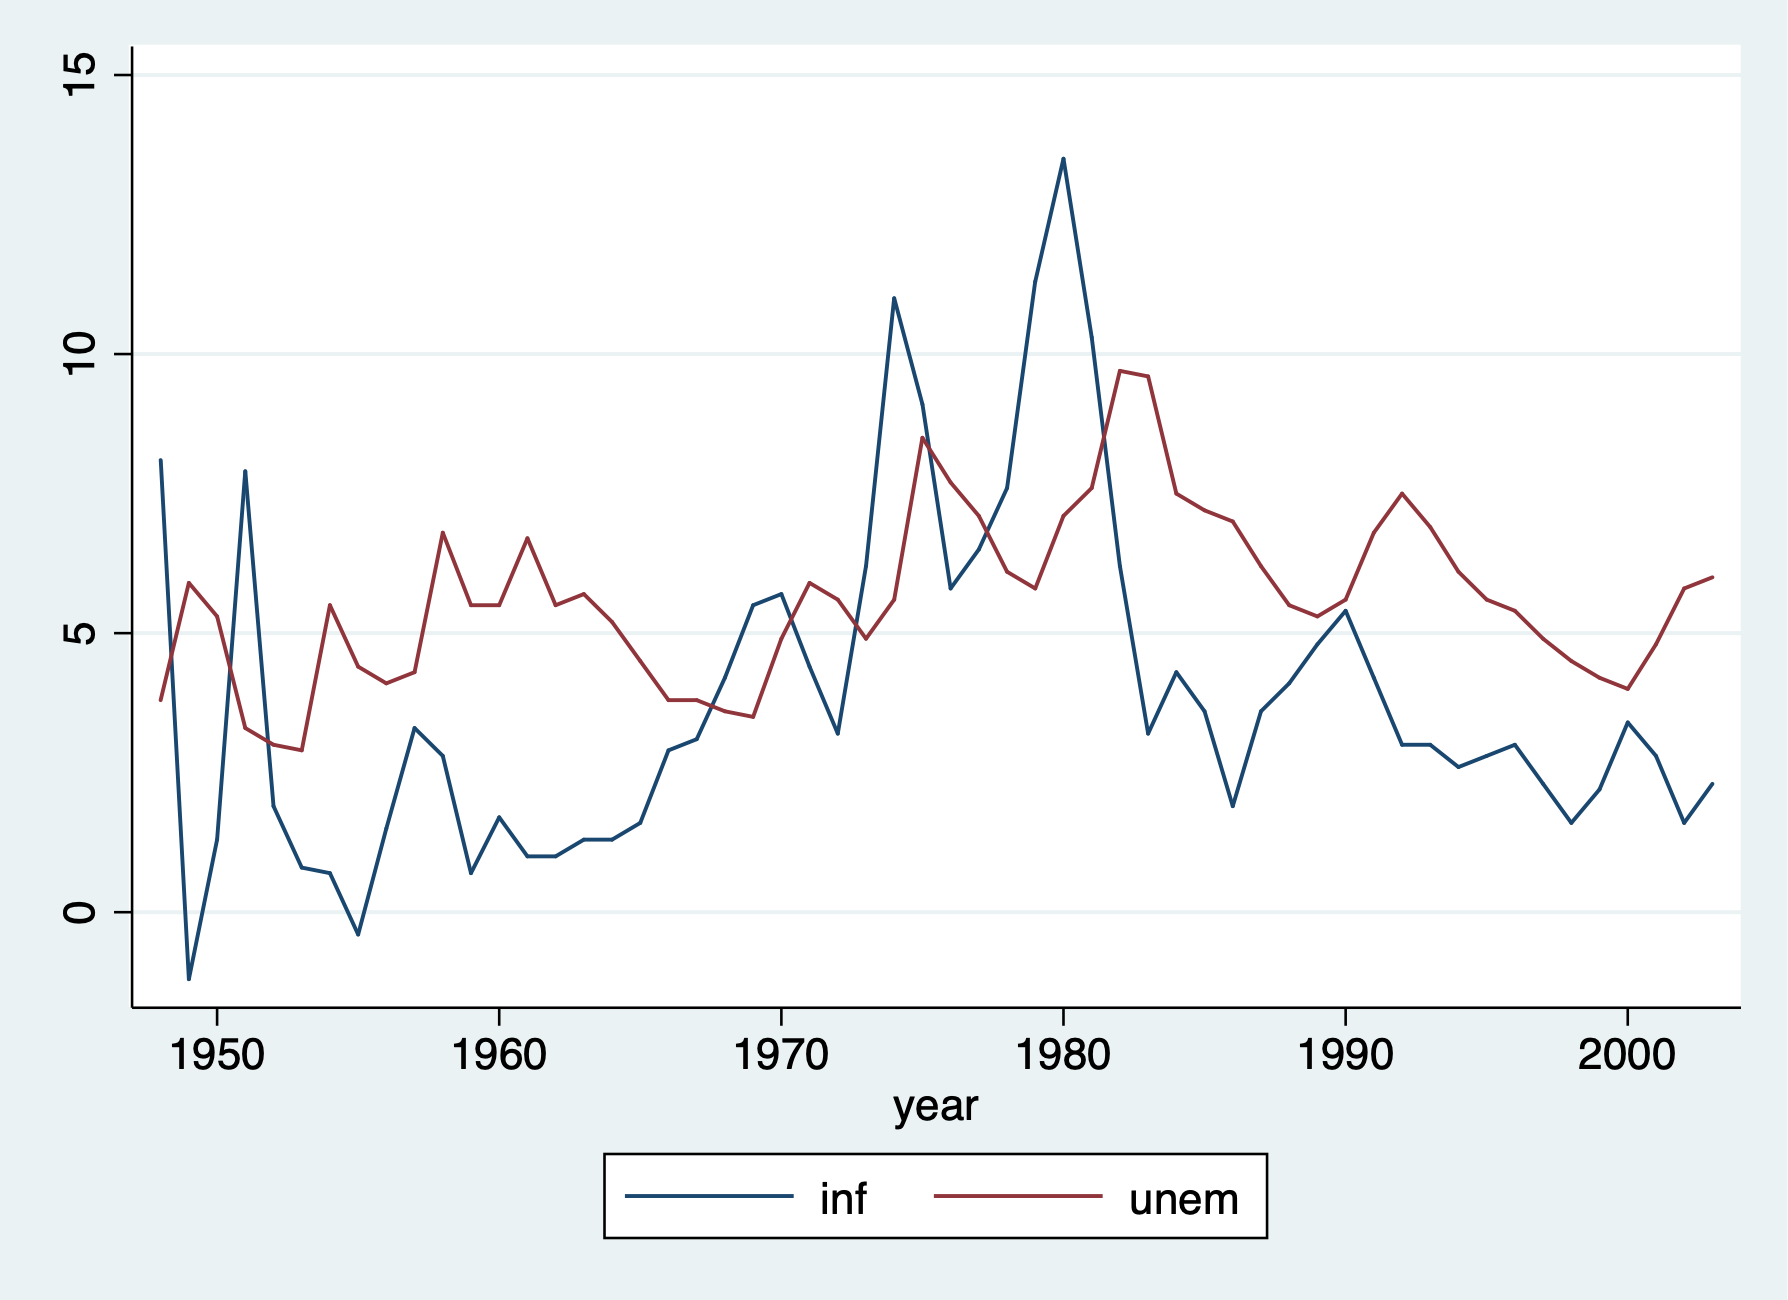
\includegraphics[keepaspectratio]{week_10_ts_infemp.png}}
\caption{TSLINE graph of inflation and unemployment}
\end{figure}

We can take the difference in the time series as well. Use the \emph{s.} operator instead of \emph{d.}. While \emph{s1} and \emph{d1} will produce similar results, \emph{s2} and \emph{d2} will not produce the same results.

\begin{Shaded}
\begin{Highlighting}[]
\KeywordTok{tsline} \FunctionTok{s}\NormalTok{.inf }\FunctionTok{s}\NormalTok{.unem}
\KeywordTok{graph} \KeywordTok{export} \StringTok{"/Users/Sam/Desktop/Econ 645/Stata/week\_10\_ts\_Dinfemp.png"}\NormalTok{, }\KeywordTok{replace}
\end{Highlighting}
\end{Shaded}

\begin{figure}
\centering
\pandocbounded{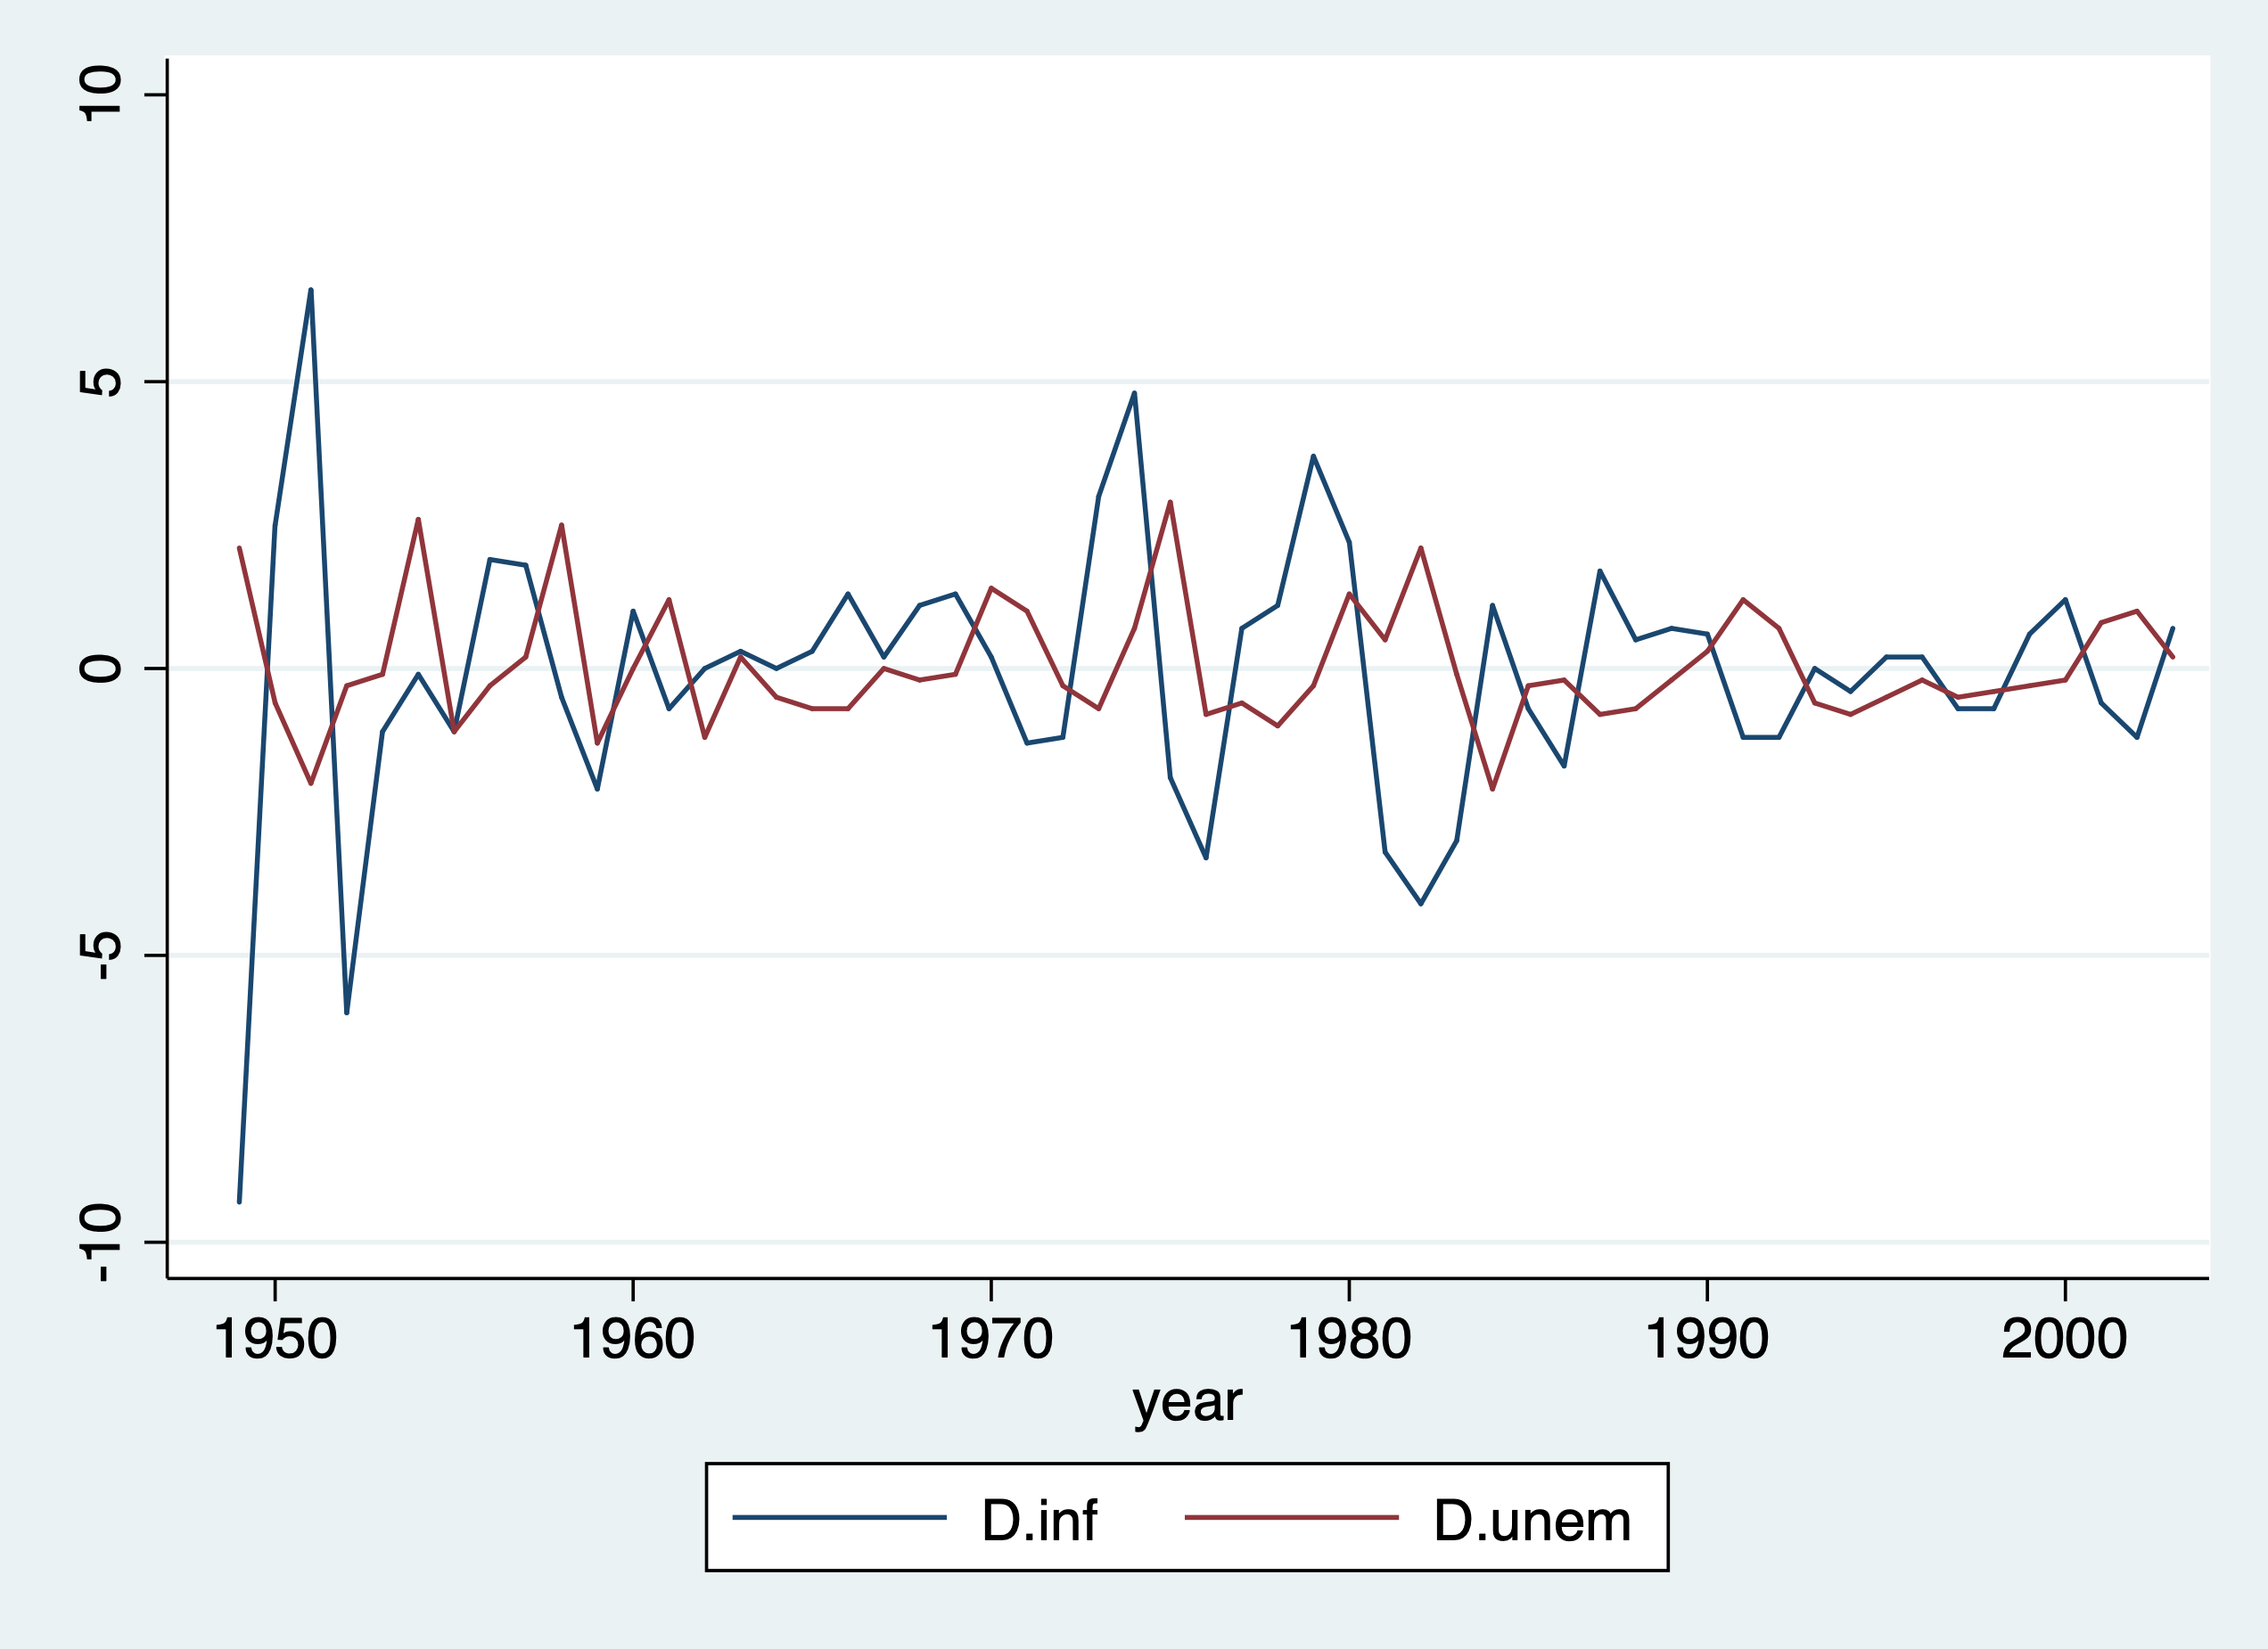
\includegraphics[keepaspectratio]{week_10_ts_Dinfemp.png}}
\caption{TSLINE graph of first difference in inflation and unemployment}
\end{figure}

\textbf{Caution}: \[ D2. \neq S2. \]
It is not recommended to use d. beyond the first difference.
Use the S12. operator If you are interested in \[ x_{t}-x_{t-12} = \Delta x \]
\emph{D2} gives the difference in differences (not the research design. Such that the \emph{D2.}operator calculates: \[ D2 = x_{t} - x_{t-1} - (x_{t-1}-x_{t-2}) \]
\[ S2 = x_{t} - x_{t-2} \]

We can take the 12-month difference in the time series as well.

\begin{Shaded}
\begin{Highlighting}[]
\KeywordTok{tsline}\NormalTok{ s2.inf s2.unem}
\KeywordTok{graph} \KeywordTok{export} \StringTok{"/Users/Sam/Desktop/Econ 645/Stata/week\_10\_ts\_D12infemp.png"}\NormalTok{, }\KeywordTok{replace}
\end{Highlighting}
\end{Shaded}

\begin{figure}
\centering
\pandocbounded{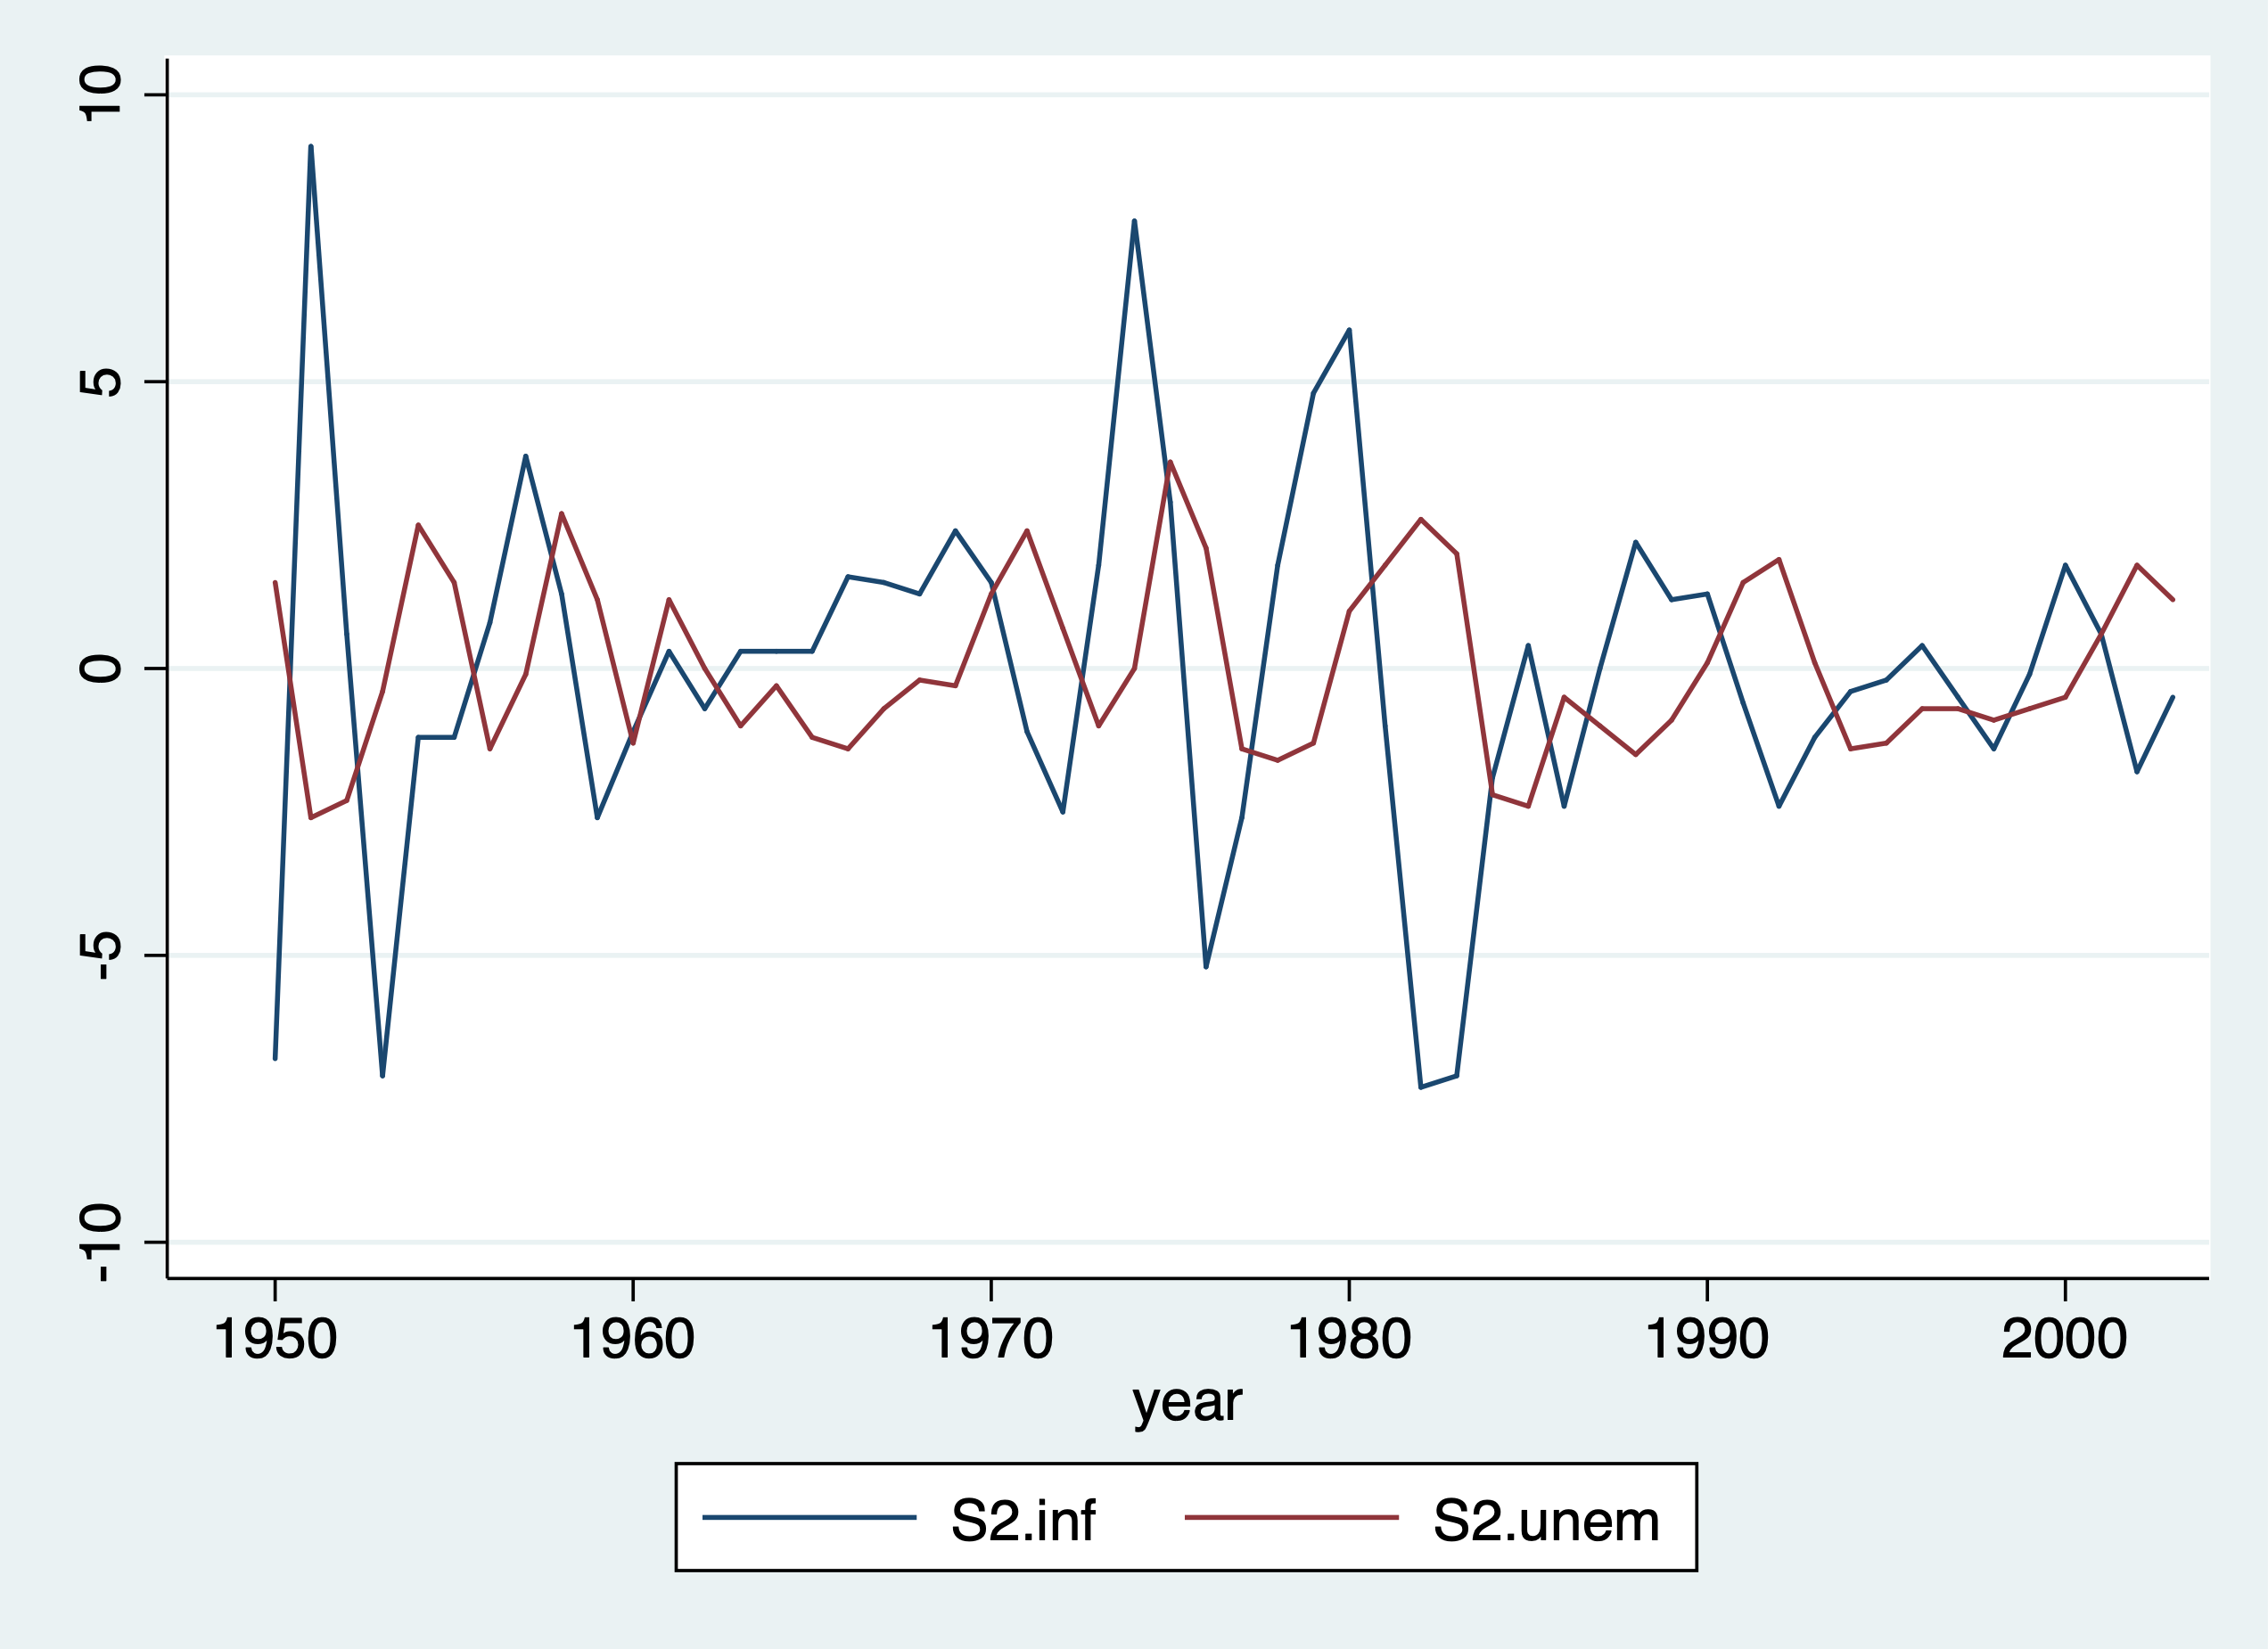
\includegraphics[keepaspectratio]{week_10_ts_D2infemp.png}}
\caption{TSLINE graph of 2-year difference in inflation and unemployment}
\end{figure}

\section{Inflation and Deficits on Interest Rates}\label{inflation-and-deficits-on-interest-rates}

\textbf{Lesson:} some static models explain time-series better than the prior model

Looking inflation and deficits on interest rates, our model is:
\[ i3_t = \beta_0 + \beta_1 inflation_t + \beta_2 deficitpct_t + u_t \]
Where

\begin{enumerate}
\def\labelenumi{\arabic{enumi}.}
\tightlist
\item
  i3: the 3-month T-bill rate
\item
  inf: the annual inflation rate from CPI
\item
  def: is the federal budget deficit as a percentage of GDP
\end{enumerate}

Set the Time Series

\begin{Shaded}
\begin{Highlighting}[]
\NormalTok{cd }\StringTok{"/Users/Sam/Desktop/Econ 645/Data/Wooldridge"}
\KeywordTok{use}\NormalTok{ intdef.dta, }\KeywordTok{clear}
\KeywordTok{tsset} \FunctionTok{year}
\KeywordTok{reg}\NormalTok{ i3 inf def }\KeywordTok{if} \FunctionTok{year}\NormalTok{ \textless{} 2004}
\end{Highlighting}
\end{Shaded}

\begin{verbatim}
/Users/Sam/Desktop/Econ 645/Data/Wooldridge

        time variable:  year, 1948 to 2003
                delta:  1 unit

      Source |       SS           df       MS      Number of obs   =        56
-------------+----------------------------------   F(2, 53)        =     40.09
       Model |  272.420338         2  136.210169   Prob > F        =    0.0000
    Residual |  180.054275        53  3.39725047   R-squared       =    0.6021
-------------+----------------------------------   Adj R-squared   =    0.5871
       Total |  452.474612        55  8.22681113   Root MSE        =    1.8432

------------------------------------------------------------------------------
          i3 |      Coef.   Std. Err.      t    P>|t|     [95% Conf. Interval]
-------------+----------------------------------------------------------------
         inf |   .6058659   .0821348     7.38   0.000     .4411243    .7706074
         def |   .5130579   .1183841     4.33   0.000     .2756095    .7505062
       _cons |   1.733266    .431967     4.01   0.000     .8668497    2.599682
------------------------------------------------------------------------------
\end{verbatim}

This static model better explain interest rates based on basic macroeconomics.
Both contemporaneous variables explain current interest rates. A 1 percentage
point increase in the inflation rate leads to a 0.6 percentage point increase
in the nominal interest rate. A 1 percentage point increase in the deficits as
a percentage of GDP leads to a 0.5 percentage point increase in nominal interest
rates.

\section{Puerto Rican Employment and Minimum Wage}\label{puerto-rican-employment-and-minimum-wage}

We'll look at the association between employment and minimum wage in Puerto Rico.
Our model will be:
\[ lprepop_t = \beta_0 + \beta_1 lmincov_t + \beta_2 lusgnp + u_t \]
Where

\begin{enumerate}
\def\labelenumi{\arabic{enumi}.}
\tightlist
\item
  ln(prepop): the natural log of the employment to population ratio in PR
\item
  ln(mincov): natural log of the importance of minimum wage relative to average wages or mincov=average minimum wage/average wages)*average coverage rate or people actually covered by the minimum wage law
\item
  lusgnp: natural log of US GNP
\end{enumerate}

Set Time Series

\begin{Shaded}
\begin{Highlighting}[]
\NormalTok{cd }\StringTok{"/Users/Sam/Desktop/Econ 645/Data/Wooldridge"}
\KeywordTok{use}\NormalTok{ prminwge, }\KeywordTok{clear}
\KeywordTok{tsset} \FunctionTok{year}
\KeywordTok{reg}\NormalTok{ lprepop lmincov lusgnp }\KeywordTok{if} \FunctionTok{year}\NormalTok{ \textless{} 1988}
\end{Highlighting}
\end{Shaded}

\begin{verbatim}
/Users/Sam/Desktop/Econ 645/Data/Wooldridge

        time variable:  year, 1950 to 1987
                delta:  1 unit

      Source |       SS           df       MS      Number of obs   =        38
-------------+----------------------------------   F(2, 35)        =     34.04
       Model |  .211258366         2  .105629183   Prob > F        =    0.0000
    Residual |  .108600151        35  .003102861   R-squared       =    0.6605
-------------+----------------------------------   Adj R-squared   =    0.6411
       Total |  .319858518        37  .008644825   Root MSE        =     .0557

------------------------------------------------------------------------------
     lprepop |      Coef.   Std. Err.      t    P>|t|     [95% Conf. Interval]
-------------+----------------------------------------------------------------
     lmincov |  -.1544442   .0649015    -2.38   0.023    -.2862011   -.0226872
      lusgnp |  -.0121888   .0885134    -0.14   0.891    -.1918806     .167503
       _cons |  -1.054423   .7654065    -1.38   0.177     -2.60828    .4994351
------------------------------------------------------------------------------
\end{verbatim}

Our results show that there is a tradeoff between the employment ratio and
the importance of minimum wage. A one percent increase in importance of
minimum wage the employment-population ratio declines .154 percent.

\section{Antidumping Filings and Chemical Imports}\label{antidumping-filings-and-chemical-imports}

The barium industry in the U.S. complained to the International Trade Commission
that China was dumping (or selling imports at lower prices to undercut domestic producers).
First, are imports unusually high before the complaint? Second, do imports
change after the dumping complaint?

Our model is the
\[ lchnimp_t = \beta_0 + \beta_1 lchempi_t + \beta_2 lgas_t + \beta_3 lrtwex_t +\beta_4 befile6_t + \beta_5 affile6_t + \beta_6 afdec6 + u_t \]

Where

\begin{enumerate}
\def\labelenumi{\arabic{enumi}.}
\tightlist
\item
  lchnimp: natural log of the volume of Chinese imports of barium chloride
\item
  lchempi: natural log of domestic chemical production index
\item
  lgas: natural log of gasoline production
\item
  lrtwex: natural log of the exchange rate index
\item
  befile6: binary for 6 months before a complaint filing
\item
  affile6: binary for 6 months after a complaint filing
\item
  afdec6: binary for 6 months after a positive decision
\end{enumerate}

Set Time Series Monthly

\begin{Shaded}
\begin{Highlighting}[]
\NormalTok{cd }\StringTok{"/Users/Sam/Desktop/Econ 645/Data/Wooldridge"}
\KeywordTok{use}\NormalTok{ barium.dta, }\KeywordTok{clear}
\KeywordTok{tsset}\NormalTok{ t, }\FunctionTok{monthly}
\KeywordTok{reg}\NormalTok{ lchnimp lchempi lgas lrtwex befile6 affile6 afdec6}
\end{Highlighting}
\end{Shaded}

\begin{verbatim}
/Users/Sam/Desktop/Econ 645/Data/Wooldridge

        time variable:  t, 1960m2 to 1970m12
                delta:  1 month

      Source |       SS           df       MS      Number of obs   =       131
-------------+----------------------------------   F(6, 124)       =      9.06
       Model |  19.4051607         6  3.23419346   Prob > F        =    0.0000
    Residual |  44.2470875       124  .356831351   R-squared       =    0.3049
-------------+----------------------------------   Adj R-squared   =    0.2712
       Total |  63.6522483       130  .489632679   Root MSE        =    .59735

------------------------------------------------------------------------------
     lchnimp |      Coef.   Std. Err.      t    P>|t|     [95% Conf. Interval]
-------------+----------------------------------------------------------------
     lchempi |   3.117193   .4792021     6.50   0.000     2.168718    4.065668
        lgas |   .1963504   .9066172     0.22   0.829    -1.598099      1.9908
      lrtwex |   .9830183   .4001537     2.46   0.015     .1910022    1.775034
     befile6 |   .0595739   .2609699     0.23   0.820    -.4569585    .5761064
     affile6 |  -.0324064   .2642973    -0.12   0.903    -.5555249     .490712
      afdec6 |   -.565245   .2858352    -1.98   0.050    -1.130993    .0005028
       _cons |    -17.803   21.04537    -0.85   0.399    -59.45769    23.85169
------------------------------------------------------------------------------
\end{verbatim}

We see that imports are not higher 6 months before a complaint, and imports
are not lower 6 months after a complaint. However, imports are lower 6 months
after a positive decision in a complaint by the ITC. The impact is fairly large
and imports of barium chloride fall about 43.2\% after a positive decision.

Also notice that rtwex is positive, and we would expect that a stronger dollar
increase demand for imports, which is about uni-elastic.

\begin{Shaded}
\begin{Highlighting}[]
\KeywordTok{display}\NormalTok{ (}\FunctionTok{exp}\NormalTok{({-}.565){-}1)*100}
\end{Highlighting}
\end{Shaded}

\begin{verbatim}
-43.163985
\end{verbatim}

\chapter{Finite Distributed Lags Models}\label{finite-distributed-lags-models}

\section{Personal Exemption on Fertility Rates}\label{personal-exemption-on-fertility-rates}

\textbf{Lesson:} using lags in the explanatory variables

Our interest the general fertility rate, which is the number of children born
to every 1,000 women of childbearing age. PE is the average real dollar value
of the personal tax exemption and two binary variables for World War II and
the introduction of the birth control pill in 1963.

Our contemporenous model is:
\[ gfr_t=\beta_0 + \beta_1 pe_t + \beta_2 ww2_t + \beta_3 pill_t + u_t \]

Where

\begin{enumerate}
\def\labelenumi{\arabic{enumi}.}
\tightlist
\item
  gfr: the fertility rate or births per 1,000 women at time t
\item
  pe: the personal tax exemptions at time t
\item
  ww2: a binary for World War II
\item
  pill: a binary for birth control pill
\end{enumerate}

Set Time Series

\begin{Shaded}
\begin{Highlighting}[]
\NormalTok{cd }\StringTok{"/Users/Sam/Desktop/Econ 645/Data/Wooldridge"}
\KeywordTok{use}\NormalTok{ fertil3.dta, }\KeywordTok{clear}
\KeywordTok{tsset} \FunctionTok{year}\NormalTok{, }\FunctionTok{yearly}
\KeywordTok{reg}\NormalTok{ gfr pe i.ww2 i.pill }\KeywordTok{if} \FunctionTok{year}\NormalTok{ \textless{} 1985}
\end{Highlighting}
\end{Shaded}

\begin{verbatim}
/Users/Sam/Desktop/Econ 645/Data/Wooldridge

        time variable:  year, 1913 to 1984
                delta:  1 year

      Source |       SS           df       MS      Number of obs   =        72
-------------+----------------------------------   F(3, 68)        =     20.38
       Model |  13183.6215         3  4394.54049   Prob > F        =    0.0000
    Residual |  14664.2739        68  215.651087   R-squared       =    0.4734
-------------+----------------------------------   Adj R-squared   =    0.4502
       Total |  27847.8954        71  392.223879   Root MSE        =    14.685

------------------------------------------------------------------------------
         gfr |      Coef.   Std. Err.      t    P>|t|     [95% Conf. Interval]
-------------+----------------------------------------------------------------
          pe |     .08254   .0296462     2.78   0.007     .0233819    .1416981
       1.ww2 |   -24.2384   7.458253    -3.25   0.002    -39.12111   -9.355684
      1.pill |  -31.59403   4.081068    -7.74   0.000    -39.73768   -23.45039
       _cons |   98.68176   3.208129    30.76   0.000     92.28003    105.0835
------------------------------------------------------------------------------
\end{verbatim}

World War II reduced the fertility rate by 24.24 births per 1,000 women of
child bearing age, while the introduction of the birth control pill reduced
the number of birth by 31.59 births per 1,000 women of childbearing age.
The personal tax exemption. A one dollar increase in the average real value of
the personal tax exemption increases 0.083 births per 1,000 women of child
bearing age or a 12 dollar increase in the average real personal
tax exemption increases 1 child per 1,000 women of child bearing ago

Next lets add lags in the average real value of the personal tax exemption.
Our Finite Distributed Lag model is:
\[ gfr_t=\beta_0 + \beta_1 pe_t + \beta_2 pe_{t-1} + \beta_3 pe_{t-2} + \beta_4 ww2_t + \beta_5 pill_t + u_t \]

\begin{Shaded}
\begin{Highlighting}[]
\KeywordTok{reg}\NormalTok{ gfr pe pe\_1 pe\_2 i.ww2 i.pill }\KeywordTok{if} \FunctionTok{year}\NormalTok{ \textless{} 1985}
\end{Highlighting}
\end{Shaded}

Our personal exemption variables are no longer statistically significiant, but
let's test the joint significance. We might have multicollinearity that bias
our standard errors for our PE variables.

\begin{Shaded}
\begin{Highlighting}[]
\NormalTok{test pe pe\_1 pe\_2}
\NormalTok{test pe\_1 pe\_2}
\end{Highlighting}
\end{Shaded}

Our PE variables are jointly significant, but our lags are jointly insignificiant
so we'll use our static model.

For the estimated LRP: \[ .073-.0058+0.034 \approx .101, \] but we lack a standard error.
We'll need to estimate the standard error.
Let \[ \theta_0=\delta_0+\delta_1+\delta_2 \] denote the LRP and write \[ \delta_0 \]
in terms of \[ \theta_0 \, , \delta_1 \, and \, \delta_2 \, where \, \delta_0 = \theta_0 - \delta_1 - \delta_2 \]
Next substitute for \[ \delta_0 \]
\[ gfr_t = \alpha_0 + \delta_0 pe_t + \delta_1 pe_{t-1} + \delta_2 pe_{t-2} + ... \]
to get
\[ gfr_t = \alpha_0 + (\theta_0 - \delta_1 - \delta_2)pe_t + \delta_1 pe_{t-1} + \delta_2 pe_{t-2} + ... \]
\[ gfr_t = \alpha_0 + \theta_0 pe_t + \delta_1 (pe_{t-1} - pe_t) + \delta_2 (pe_{t-2} - pe_t) + \]

We can estimate \[ \hat{\theta}_{0} \] and its standard error.
We can regress gfr\_t onto pe\_t, (pe\_(t-1) - pe\_t), and (pe\_t-2 - pe\_t), ww2, and pill

\begin{Shaded}
\begin{Highlighting}[]
    \KeywordTok{gen}\NormalTok{ pe\_1\_1 = pe\_1 {-} pe}
    \KeywordTok{gen}\NormalTok{ pe\_2\_1 = pe\_2 {-} pe}
    \KeywordTok{reg}\NormalTok{ gfr pe pe\_1\_1 pe\_2\_1 i.ww2 i.pill}
\end{Highlighting}
\end{Shaded}

\(\hat{\theta} \approx 0.101\) and significant, so our LRP has an effect on general fertility rates.

\chapter{Time Trends}\label{time-trends}

\section{Housing Investment and Housing Prices}\label{housing-investment-and-housing-prices}

\textbf{Lesson:} Importance of time trends

We look at annual housing investement and a housing price index from 1947 to 1988.

Set Time Series

\begin{Shaded}
\begin{Highlighting}[]
\NormalTok{cd }\StringTok{"/Users/Sam/Desktop/Econ 645/Data/Wooldridge"}
\KeywordTok{use}\NormalTok{ hseinv.dta, }\KeywordTok{clear}
\KeywordTok{tsset} \FunctionTok{year}\NormalTok{, }\FunctionTok{yearly}
\end{Highlighting}
\end{Shaded}

\begin{verbatim}
/Users/Sam/Desktop/Econ 645/Data/Wooldridge

        time variable:  year, 1947 to 1988
                delta:  1 year
\end{verbatim}

Our model is the natural log of invpc or real per capita housing investment (\$1,000)
and price be the housing price index where 1982 = 1 (or 100). We'll assume
constant elasticity with our log-log model.

\[ linvpc_t = \beta_0 + \beta_1 lprice_t + u_t \]

\begin{Shaded}
\begin{Highlighting}[]
\KeywordTok{reg}\NormalTok{ linvpc lprice}
\end{Highlighting}
\end{Shaded}

\begin{verbatim}
      Source |       SS           df       MS      Number of obs   =        42
-------------+----------------------------------   F(1, 40)        =     10.53
       Model |  .254364468         1  .254364468   Prob > F        =    0.0024
    Residual |  .966255566        40  .024156389   R-squared       =    0.2084
-------------+----------------------------------   Adj R-squared   =    0.1886
       Total |  1.22062003        41   .02977122   Root MSE        =    .15542

------------------------------------------------------------------------------
      linvpc |      Coef.   Std. Err.      t    P>|t|     [95% Conf. Interval]
-------------+----------------------------------------------------------------
      lprice |   1.240943   .3824192     3.24   0.002     .4680452    2.013841
       _cons |  -.5502345   .0430266   -12.79   0.000    -.6371945   -.4632746
------------------------------------------------------------------------------
\end{verbatim}

Our output shows that a 1 percent increase in the pricing index increases
the investment per capita by 1.24 percent (or elastic response).
Note: both investment and price have upward trends that we need to account for.

\[ invpc_t = \beta_0 + \beta_1 lprice_t + \beta_2 t + u_t \]

\begin{Shaded}
\begin{Highlighting}[]
\KeywordTok{reg}\NormalTok{ linvpc lprice t}
\end{Highlighting}
\end{Shaded}

\begin{verbatim}
      Source |       SS           df       MS      Number of obs   =        42
-------------+----------------------------------   F(2, 39)        =     10.08
       Model |  .415945108         2  .207972554   Prob > F        =    0.0003
    Residual |  .804674927        39   .02063269   R-squared       =    0.3408
-------------+----------------------------------   Adj R-squared   =    0.3070
       Total |  1.22062003        41   .02977122   Root MSE        =    .14364

------------------------------------------------------------------------------
      linvpc |      Coef.   Std. Err.      t    P>|t|     [95% Conf. Interval]
-------------+----------------------------------------------------------------
      lprice |  -.3809612   .6788352    -0.56   0.578    -1.754035    .9921125
           t |   .0098287   .0035122     2.80   0.008     .0027246    .0169328
       _cons |  -.9130595   .1356133    -6.73   0.000    -1.187363   -.6387557
------------------------------------------------------------------------------
\end{verbatim}

After accounting for the upward linear trend for both investment per capita and
the housing price index, an increase in price is coefficient is now negative, but
it is not statistically significant. We probably have serial correlation which
will bias our standard errors.

\begin{Shaded}
\begin{Highlighting}[]
\KeywordTok{predict}\NormalTok{ u, }\KeywordTok{resid}
\KeywordTok{reg}\NormalTok{ u }\OtherTok{l}\NormalTok{.u, noconst}
\KeywordTok{drop}\NormalTok{ u}
\end{Highlighting}
\end{Shaded}

\begin{verbatim}
      Source |       SS           df       MS      Number of obs   =        41
-------------+----------------------------------   F(1, 40)        =     11.10
       Model |  .170666637         1  .170666637   Prob > F        =    0.0019
    Residual |  .614779847        40  .015369496   R-squared       =    0.2173
-------------+----------------------------------   Adj R-squared   =    0.1977
       Total |  .785446484        41  .019157231   Root MSE        =    .12397

------------------------------------------------------------------------------
           u |      Coef.   Std. Err.      t    P>|t|     [95% Conf. Interval]
-------------+----------------------------------------------------------------
           u |
         L1. |   .4632581   .1390204     3.33   0.002     .1822874    .7442288
------------------------------------------------------------------------------
\end{verbatim}

\section{Personal Exemption on Fertility Rates}\label{personal-exemption-on-fertility-rates-1}

\textbf{Lesson:} Importance of non-linear time trends

We'll look at fertility again, but we'll account for a quadratic time trend.
First, we'll estimate a linear time trend, and then we'll try a quadratic time trend.

Set Time Series

\begin{Shaded}
\begin{Highlighting}[]
\NormalTok{cd }\StringTok{"/Users/Sam/Desktop/Econ 645/Data/Wooldridge"}
\KeywordTok{use}\NormalTok{ fertil3.dta, }\KeywordTok{clear}
\KeywordTok{tsset} \FunctionTok{year}\NormalTok{, }\FunctionTok{yearly}
\end{Highlighting}
\end{Shaded}

\begin{verbatim}
/Users/Sam/Desktop/Econ 645/Data/Wooldridge

        time variable:  year, 1913 to 1984
                delta:  1 year
\end{verbatim}

Linear Trend

\begin{Shaded}
\begin{Highlighting}[]
\KeywordTok{reg}\NormalTok{ gfr pe i.ww2 i.pill t }\KeywordTok{if} \FunctionTok{year}\NormalTok{ \textless{} 1985}
\end{Highlighting}
\end{Shaded}

\begin{verbatim}
      Source |       SS           df       MS      Number of obs   =        72
-------------+----------------------------------   F(4, 67)        =     32.84
       Model |  18441.2357         4  4610.30894   Prob > F        =    0.0000
    Residual |  9406.65967        67  140.397905   R-squared       =    0.6622
-------------+----------------------------------   Adj R-squared   =    0.6420
       Total |  27847.8954        71  392.223879   Root MSE        =    11.849

------------------------------------------------------------------------------
         gfr |      Coef.   Std. Err.      t    P>|t|     [95% Conf. Interval]
-------------+----------------------------------------------------------------
          pe |   .2788778   .0400199     6.97   0.000     .1989978    .3587578
       1.ww2 |  -35.59228   6.297377    -5.65   0.000     -48.1619   -23.02266
      1.pill |   .9974479    6.26163     0.16   0.874    -11.50082    13.49571
           t |  -1.149872   .1879038    -6.12   0.000    -1.524929   -.7748145
       _cons |   111.7694   3.357765    33.29   0.000     105.0673    118.4716
------------------------------------------------------------------------------
\end{verbatim}

Quadratic Trend
Fertility is declining but at a decreasing negatively rate (eventually a positive t\^{}2 takes over t)

\begin{Shaded}
\begin{Highlighting}[]
\KeywordTok{reg}\NormalTok{ gfr pe i.ww2 i.pill c.t\#\#c.t }\KeywordTok{if} \FunctionTok{year}\NormalTok{ \textless{} 1985}
\end{Highlighting}
\end{Shaded}

\begin{verbatim}
      Source |       SS           df       MS      Number of obs   =        72
-------------+----------------------------------   F(5, 66)        =     35.09
       Model |  20236.3981         5  4047.27961   Prob > F        =    0.0000
    Residual |  7611.49734        66  115.325717   R-squared       =    0.7267
-------------+----------------------------------   Adj R-squared   =    0.7060
       Total |  27847.8954        71  392.223879   Root MSE        =    10.739

------------------------------------------------------------------------------
         gfr |      Coef.   Std. Err.      t    P>|t|     [95% Conf. Interval]
-------------+----------------------------------------------------------------
          pe |   .3478126   .0402599     8.64   0.000     .2674311     .428194
       1.ww2 |  -35.88028   5.707921    -6.29   0.000    -47.27651   -24.48404
      1.pill |  -10.11972   6.336094    -1.60   0.115    -22.77014    2.530696
           t |  -2.531426   .3893863    -6.50   0.000    -3.308861   -1.753991
             |
     c.t#c.t |   .0196126    .004971     3.95   0.000     .0096876    .0295377
             |
       _cons |   124.0919   4.360738    28.46   0.000     115.3854    132.7984
------------------------------------------------------------------------------
\end{verbatim}

The fertility rate exhibits upward and downward trends between 1913 and 1984.
Interestingly, pe remains fairly robust after adding time trends. The linear
time trend shows that general fertility rates are falling by 1.15 childs per 1,000
women of childbearing age for each additional year. However, the quadratic shows
that the trend is negative but decreasing rate and will eventually become positive.

\section{Puerto Rican Employment}\label{puerto-rican-employment}

The last linear trend is for employment-population ratio and the importance of minimum wage
coverage. We'll add a time trend along with mincov and usgnp.

Set the Time Series

\begin{Shaded}
\begin{Highlighting}[]
\NormalTok{cd }\StringTok{"/Users/Sam/Desktop/Econ 645/Data/Wooldridge"}
\KeywordTok{use}\NormalTok{ prminwge, }\KeywordTok{clear}
\KeywordTok{tsset} \FunctionTok{year}\NormalTok{, }\FunctionTok{yearly}
\end{Highlighting}
\end{Shaded}

\begin{verbatim}
/Users/Sam/Desktop/Econ 645/Data/Wooldridge

        time variable:  year, 1950 to 1987
                delta:  1 year
\end{verbatim}

Add linear trend

\begin{Shaded}
\begin{Highlighting}[]
\KeywordTok{reg}\NormalTok{ lprepop lmincov lusgnp t}
\end{Highlighting}
\end{Shaded}

\begin{verbatim}
      Source |       SS           df       MS      Number of obs   =        38
-------------+----------------------------------   F(3, 34)        =     62.78
       Model |  .270948453         3  .090316151   Prob > F        =    0.0000
    Residual |  .048910064        34  .001438531   R-squared       =    0.8471
-------------+----------------------------------   Adj R-squared   =    0.8336
       Total |  .319858518        37  .008644825   Root MSE        =    .03793

------------------------------------------------------------------------------
     lprepop |      Coef.   Std. Err.      t    P>|t|     [95% Conf. Interval]
-------------+----------------------------------------------------------------
     lmincov |  -.1686949   .0442463    -3.81   0.001    -.2586142   -.0787757
      lusgnp |   1.057351   .1766369     5.99   0.000     .6983813     1.41632
           t |  -.0323542   .0050227    -6.44   0.000    -.0425616   -.0221468
       _cons |  -8.696298   1.295764    -6.71   0.000    -11.32961   -6.062988
------------------------------------------------------------------------------
\end{verbatim}

The employment-population ratio does not have much of a downward or upward trend,
but usgnp does. Тhe linear trend of usgnp is about 3\% per year, so an estimate
of 1.06 in our model mean that when usgnp increases by 1\% above its long-term
trend, employment-population ratio increases by about 1.06\%

\chapter{Seasonality}\label{seasonality}

We'll add monthly variables to account for the fact that imports are not
seasonlly adjusted.

Set Time Series Monthly

\begin{Shaded}
\begin{Highlighting}[]
\NormalTok{cd }\StringTok{"/Users/Sam/Desktop/Econ 645/Data/Wooldridge"}
\KeywordTok{use}\NormalTok{ barium.dta, }\KeywordTok{clear}
\KeywordTok{tsset}\NormalTok{ t, }\FunctionTok{monthly}
\KeywordTok{reg}\NormalTok{ lchnimp lchempi lgas lrtwex befile6 affile6 afdec6 }\CommentTok{///}
\NormalTok{  feb mar apr may jun jul aug sep oct nov dec}
\end{Highlighting}
\end{Shaded}

\begin{verbatim}
/Users/Sam/Desktop/Econ 645/Data/Wooldridge

        time variable:  t, 1960m2 to 1970m12
                delta:  1 month

      Source |       SS           df       MS      Number of obs   =       131
-------------+----------------------------------   F(17, 113)      =      3.71
       Model |  22.8083523        17  1.34166778   Prob > F        =    0.0000
    Residual |   40.843896       113  .361450407   R-squared       =    0.3583
-------------+----------------------------------   Adj R-squared   =    0.2618
       Total |  63.6522483       130  .489632679   Root MSE        =    .60121

------------------------------------------------------------------------------
     lchnimp |      Coef.   Std. Err.      t    P>|t|     [95% Conf. Interval]
-------------+----------------------------------------------------------------
     lchempi |    3.26506   .4929302     6.62   0.000     2.288476    4.241644
        lgas |  -1.278121   1.389008    -0.92   0.359    -4.029997    1.473755
      lrtwex |   .6630496   .4713038     1.41   0.162    -.2706882    1.596787
     befile6 |   .1397024   .2668075     0.52   0.602    -.3888914    .6682962
     affile6 |   .0126317   .2786866     0.05   0.964    -.5394967    .5647601
      afdec6 |  -.5213006     .30195    -1.73   0.087    -1.119518    .0769168
         feb |  -.4177089   .3044445    -1.37   0.173    -1.020868    .1854505
         mar |   .0590528   .2647308     0.22   0.824    -.4654266    .5835322
         apr |  -.4514825   .2683865    -1.68   0.095    -.9832046    .0802396
         may |   .0333085   .2692425     0.12   0.902    -.5001093    .5667264
         jun |  -.2063321   .2692515    -0.77   0.445    -.7397679    .3271038
         jul |   .0038354   .2787665     0.01   0.989    -.5484513    .5561222
         aug |  -.1570652   .2779928    -0.56   0.573    -.7078191    .3936887
         sep |  -.1341606   .2676556    -0.50   0.617    -.6644348    .3961135
         oct |   .0516921   .2668512     0.19   0.847    -.4769883    .5803725
         nov |    -.24626   .2628272    -0.94   0.351     -.766968     .274448
         dec |   .1328368   .2714234     0.49   0.626    -.4049019    .6705755
       _cons |   16.77877   32.42865     0.52   0.606    -47.46824    81.02577
------------------------------------------------------------------------------
\end{verbatim}

We compare all months to January as the base period, but let's test their
joint significance.

\begin{Shaded}
\begin{Highlighting}[]
\KeywordTok{test}\NormalTok{ feb mar apr may jun jul aug sep oct nov dec}
\end{Highlighting}
\end{Shaded}

\begin{verbatim}
 ( 1)  feb = 0
 ( 2)  mar = 0
 ( 3)  apr = 0
 ( 4)  may = 0
 ( 5)  jun = 0
 ( 6)  jul = 0
 ( 7)  aug = 0
 ( 8)  sep = 0
 ( 9)  oct = 0
 (10)  nov = 0
 (11)  dec = 0

       F( 11,   113) =    0.86
            Prob > F =    0.5852
\end{verbatim}

We find that they are jointly insignificant and seasonality does not seem
to be an issue with barium chloride imports.

\chapter{Weakly Dependent and Stationary Time Series AR(1) Models}\label{weakly-dependent-and-stationary-time-series-ar1-models}

\section{Efficient Market Hypothesis}\label{efficient-market-hypothesis}

We'll test the a version of the efficient market hypothesis (EMH) by looking
at weekly stock return from 1976 to 1989.

Set Time Series

\begin{Shaded}
\begin{Highlighting}[]
\NormalTok{cd }\StringTok{"/Users/Sam/Desktop/Econ 645/Data/Wooldridge"}
\KeywordTok{use}\NormalTok{ nyse, }\KeywordTok{clear}
\KeywordTok{tsset}\NormalTok{ t, }\FunctionTok{weekly}
\end{Highlighting}
\end{Shaded}

\begin{verbatim}
/Users/Sam/Desktop/Econ 645/Data/Wooldridge

        time variable:  t, 1960w2 to 1973w16
                delta:  1 week
\end{verbatim}

Our dependent variable is the weekly percentage return on the New York Stock Exchange.
A strict form of the EMH states that information observable to the market prior to
week t should not help to predict the return during week t.
\[ E(y_t|y_{t-1},y_{t-2},...)=E(y_t) \]

We will test EMH by specifying an AR(1) model and our hypothesis states that
beta for y\_(t-1) will be equal to 0. We'll assume that stock returns are
serially uncorrelated, so we can safetly assume that they are weakly dependent.

\[ return_t = \beta_0 + \rho return_{t-1} + e_t \]

\begin{Shaded}
\begin{Highlighting}[]
\KeywordTok{reg} \FunctionTok{return} \OtherTok{l}\NormalTok{.}\FunctionTok{return}

\NormalTok{*Or}
\KeywordTok{reg} \FunctionTok{return}\NormalTok{ return\_1}
\KeywordTok{predict}\NormalTok{ u, }\KeywordTok{resid}
\KeywordTok{reg}\NormalTok{ u }\OtherTok{l}\NormalTok{.u, noconst}
\KeywordTok{drop}\NormalTok{ u}
\end{Highlighting}
\end{Shaded}

\begin{verbatim}
      Source |       SS           df       MS      Number of obs   =       689
-------------+----------------------------------   F(1, 687)       =      2.40
       Model |  10.6866231         1  10.6866231   Prob > F        =    0.1218
    Residual |  3059.73817       687  4.45376735   R-squared       =    0.0035
-------------+----------------------------------   Adj R-squared   =    0.0020
       Total |  3070.42479       688  4.46282673   Root MSE        =    2.1104

------------------------------------------------------------------------------
      return |      Coef.   Std. Err.      t    P>|t|     [95% Conf. Interval]
-------------+----------------------------------------------------------------
      return |
         L1. |   .0588984   .0380231     1.55   0.122    -.0157569    .1335538
             |
       _cons |    .179634   .0807419     2.22   0.026     .0211034    .3381646
------------------------------------------------------------------------------

      Source |       SS           df       MS      Number of obs   =       689
-------------+----------------------------------   F(1, 687)       =      2.40
       Model |  10.6866231         1  10.6866231   Prob > F        =    0.1218
    Residual |  3059.73817       687  4.45376735   R-squared       =    0.0035
-------------+----------------------------------   Adj R-squared   =    0.0020
       Total |  3070.42479       688  4.46282673   Root MSE        =    2.1104

------------------------------------------------------------------------------
      return |      Coef.   Std. Err.      t    P>|t|     [95% Conf. Interval]
-------------+----------------------------------------------------------------
    return_1 |   .0588984   .0380231     1.55   0.122    -.0157569    .1335538
       _cons |    .179634   .0807419     2.22   0.026     .0211034    .3381646
------------------------------------------------------------------------------

(2 missing values generated)

      Source |       SS           df       MS      Number of obs   =       688
-------------+----------------------------------   F(1, 687)       =      0.00
       Model |   .00603936         1   .00603936   Prob > F        =    0.9706
    Residual |  3059.08227       687  4.45281262   R-squared       =    0.0000
-------------+----------------------------------   Adj R-squared   =   -0.0015
       Total |  3059.08831       688  4.44634929   Root MSE        =    2.1102

------------------------------------------------------------------------------
           u |      Coef.   Std. Err.      t    P>|t|     [95% Conf. Interval]
-------------+----------------------------------------------------------------
           u |
         L1. |    .001405   .0381496     0.04   0.971    -.0734987    .0763087
------------------------------------------------------------------------------
\end{verbatim}

We cannot reject the null hypothesis under our model, but we do have some
evidence of positive serial correlation.

\section{Expected Augmented Phillips Curve}\label{expected-augmented-phillips-curve}

We'll revisit the Phillips curve

Set Time Series

\begin{Shaded}
\begin{Highlighting}[]
\NormalTok{cd }\StringTok{"/Users/Sam/Desktop/Econ 645/Data/Wooldridge"}    
\KeywordTok{use}\NormalTok{ phillips.dta, }\KeywordTok{clear}
\KeywordTok{tsset} \FunctionTok{year}
\end{Highlighting}
\end{Shaded}

\begin{verbatim}
/Users/Sam/Desktop/Econ 645/Data/Wooldridge

        time variable:  year, 1948 to 2003
                delta:  1 unit
\end{verbatim}

A linear version of the expections augmented Phillips curve can be written as
\[ inf_t - inf^e_t=\beta_1(unemp_t-\mu_0) + e_t \]

Where \(mu_0\) is the natural rate of unemployment and inf\^{}e is the expected rate
of inflation formed in year t-1.
The difference between actual unemployment and the natural rate is called
cyclical unemployment, while the difference between inflation and expected
inflation is called unanticipated inflation
Our e\_t is called our supply shock.
If there is a trade-off between inflation and unemployment our \(\hat{\beta_1}\)
will be negative.

An assumption is made about inflationary expectations and unders adaptive expectations,
the expected value of current inflation depends on recently observed inflation.
The expected inflation will be assumed to be equal to last years inflation
\[ inf_t - inf_{t-1}=\beta_0 + \beta_1 unemp_t + e_t \]
\[ \Delta inf_t =\beta_0 + \beta_1 unemp_t + e_t \]

Where
\[ \Delta inf_t=inf_t - inf_{t-1} \]
\[ \beta_0 = -\beta_1 \mu_0 \]
Since beta\_1 is expected to be negative and beta\_0 is expected to be positive.

Therefore, under adaptive expectations, the augmented Phillips curve relates the
change in inflation to the level of unemployment and a supply shock e\_t.
We'll assume assumptions TSC.1-TSC.5 hold.

First Difference in the dependent variable or adaptive expectations of inflation.

\begin{Shaded}
\begin{Highlighting}[]
\KeywordTok{reg}\NormalTok{ cinf unem }\KeywordTok{if} \FunctionTok{year}\NormalTok{ \textless{} 1997}

\NormalTok{*}\KeywordTok{or}
\KeywordTok{reg} \KeywordTok{d}\NormalTok{.inf unem }\KeywordTok{if} \FunctionTok{year}\NormalTok{ \textless{} 1997}
\end{Highlighting}
\end{Shaded}

\begin{verbatim}
      Source |       SS           df       MS      Number of obs   =        48
-------------+----------------------------------   F(1, 46)        =      5.56
       Model |  33.3830007         1  33.3830007   Prob > F        =    0.0227
    Residual |  276.305134        46  6.00663335   R-squared       =    0.1078
-------------+----------------------------------   Adj R-squared   =    0.0884
       Total |  309.688135        47  6.58910925   Root MSE        =    2.4508

------------------------------------------------------------------------------
        cinf |      Coef.   Std. Err.      t    P>|t|     [95% Conf. Interval]
-------------+----------------------------------------------------------------
        unem |  -.5425869   .2301559    -2.36   0.023    -1.005867    -.079307
       _cons |   3.030581    1.37681     2.20   0.033     .2592061    5.801955
------------------------------------------------------------------------------

      Source |       SS           df       MS      Number of obs   =        48
-------------+----------------------------------   F(1, 46)        =      5.56
       Model |  33.3829996         1  33.3829996   Prob > F        =    0.0227
    Residual |  276.305138        46  6.00663344   R-squared       =    0.1078
-------------+----------------------------------   Adj R-squared   =    0.0884
       Total |  309.688138        47  6.58910932   Root MSE        =    2.4508

------------------------------------------------------------------------------
       D.inf |      Coef.   Std. Err.      t    P>|t|     [95% Conf. Interval]
-------------+----------------------------------------------------------------
        unem |  -.5425869   .2301559    -2.36   0.023    -1.005867    -.079307
       _cons |   3.030581    1.37681     2.20   0.033      .259206    5.801955
------------------------------------------------------------------------------
\end{verbatim}

The trade-off between unanticipated inflation and cyclical unemployment is
seen in \(\hat{beta_1}\). A 1-point increase in unemployment decreases unanticipated
inflation by about .54 points.

We can estimate the natural rate of unemployment by dividing \(\hat{beta_0}\) by
negative of \(\hat{beta_1}\)

\[ \mu_{0} = \hat{\beta}_{0} / - \hat{\beta}_{1} \]

\begin{Shaded}
\begin{Highlighting}[]
\KeywordTok{display}\NormalTok{ 3.03/.5425}
\end{Highlighting}
\end{Shaded}

\begin{verbatim}
5.5852535
\end{verbatim}

Plot the graph.

\begin{Shaded}
\begin{Highlighting}[]
\KeywordTok{twoway} \KeywordTok{line}\NormalTok{ cinf }\FunctionTok{year}\NormalTok{ || }\KeywordTok{line}\NormalTok{ unem }\FunctionTok{year}\NormalTok{, lpattern(}\KeywordTok{dash}\NormalTok{) }\CommentTok{///}
    \BaseNTok{legend}\NormalTok{(}\KeywordTok{order}\NormalTok{(1 }\StringTok{"Difference in Inflation"}\NormalTok{ 2 }\StringTok{"Unemployment Rate"}\NormalTok{)) }\CommentTok{///}
    \BaseNTok{title}\NormalTok{(}\StringTok{"Augmented Phillips Curve"}\NormalTok{) }\BaseNTok{ytitle}\NormalTok{(Percentage) }\BaseNTok{xtitle}\NormalTok{(}\FunctionTok{year}\NormalTok{)}
    
\KeywordTok{graph} \KeywordTok{export} \StringTok{"week\_10\_augmented\_phillips.png"}\NormalTok{, }\KeywordTok{replace}
\end{Highlighting}
\end{Shaded}

\begin{figure}
\centering
\pandocbounded{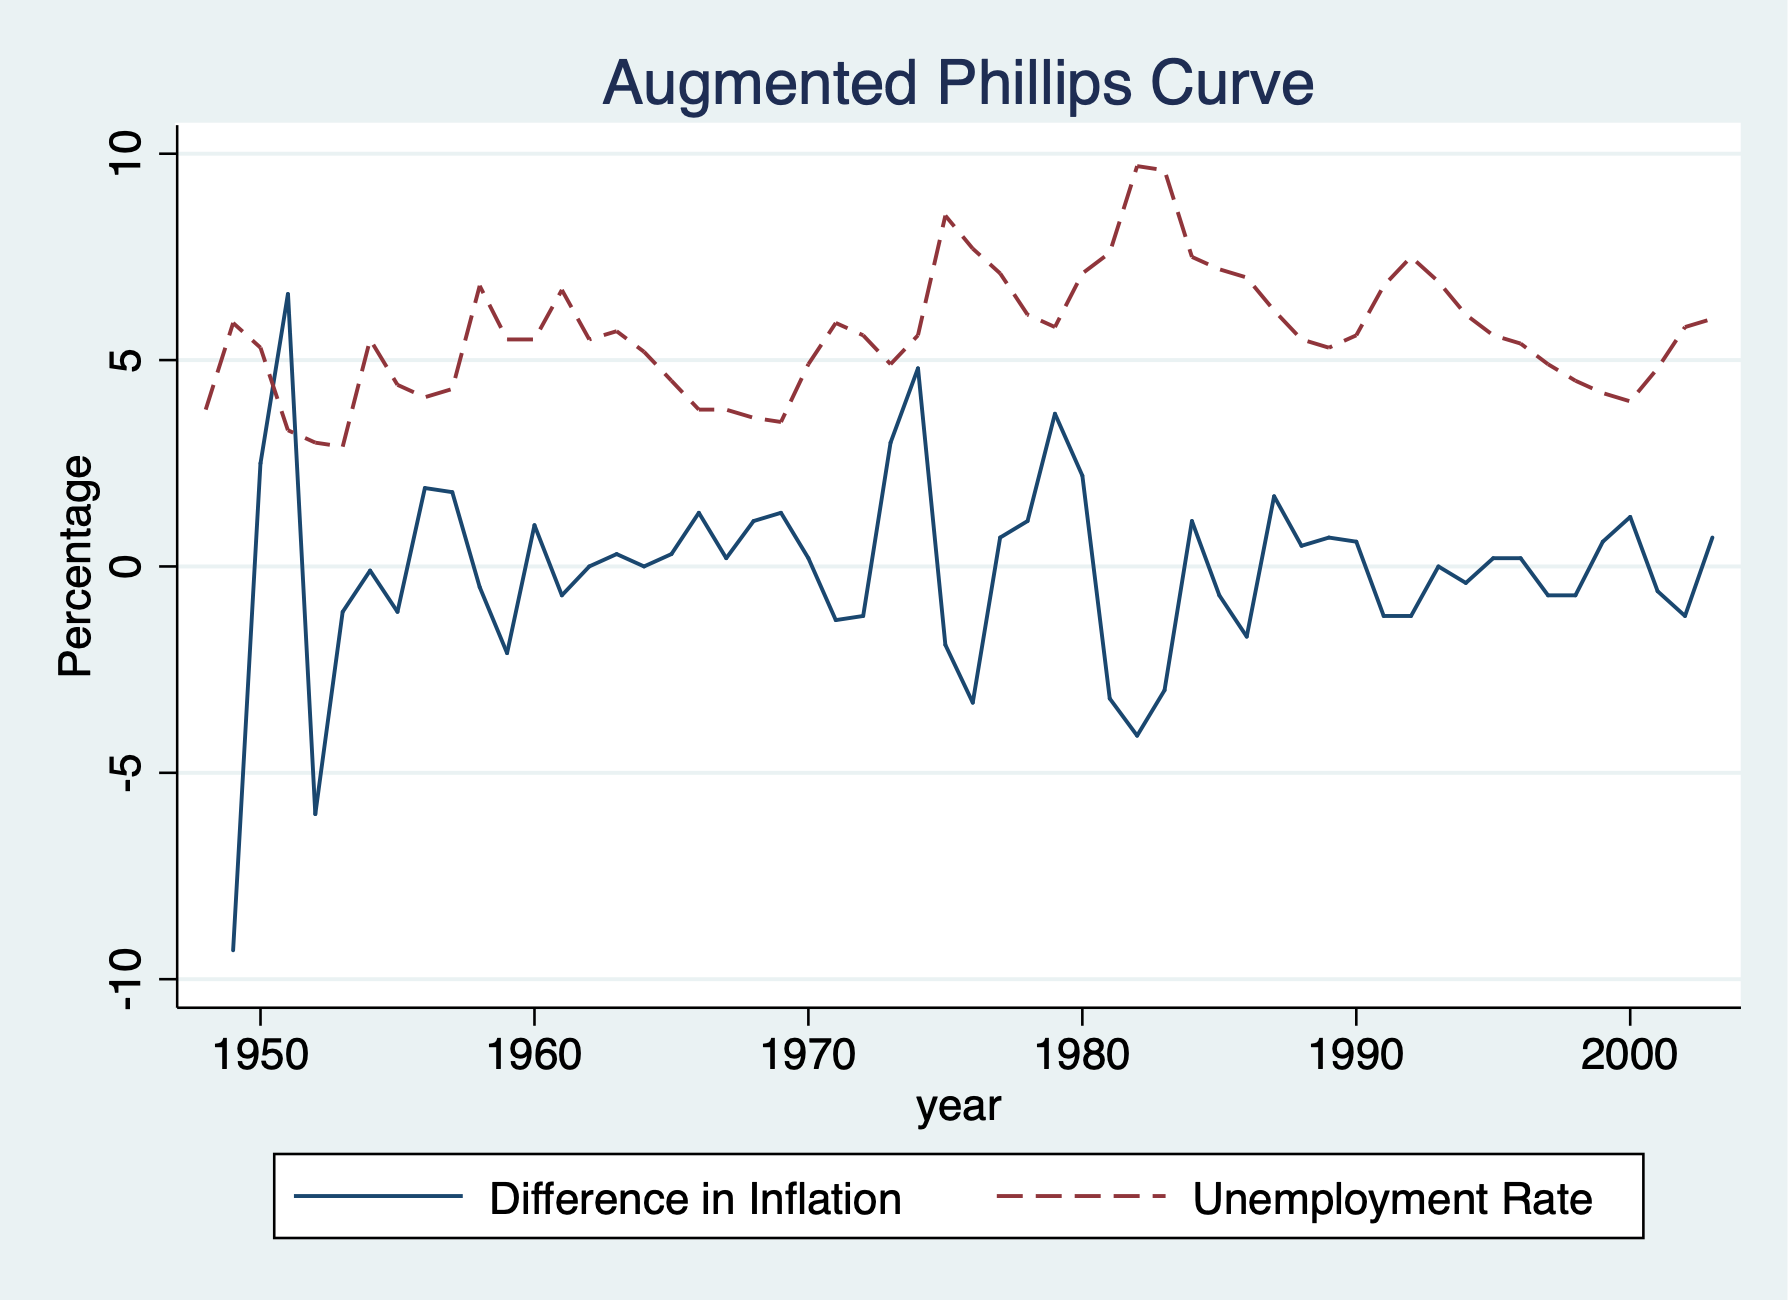
\includegraphics[keepaspectratio]{week_10_augmented_phillips.png}}
\caption{Line graph of inflation}
\end{figure}

Mitchell, N.M. (2020). \emph{Data Management Using Stata: A Practical Handbook}. (2nd ed.). Stata Press.

UCLA Advanced Research Computing. (2025). \emph{How can I access information stored after I run a command in Stata.} Retrieved from \url{https://stats.oarc.ucla.edu/stata/faq/how-can-i-access-information-stored-after-i-run-a-command-in-stata-returned-results/}

Wooldridge (2009). \emph{Introductory Econometrics: A Modern Approach}. (4th ed.). South-Western Cengage Learning.

\bibliography{book.bib,packages.bib}

\end{document}
